

\begin{figure}[H]
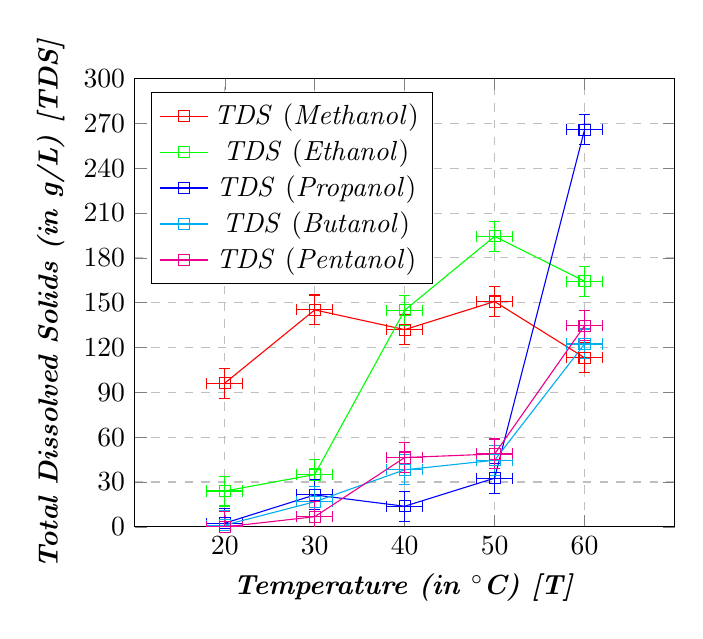
\begin{tikzpicture}
            \begin{axis}[
%                title={\textit{Graph in relation to the \textbf{experimental} \& \textbf{simulation} values of \textbf{drag force} versus \textbf{temperature}}},
                xlabel={\textbf{\textit{Temperature (in $\bm{^\circ}$C) [T]}}},
                ylabel={\textbf{\textit{Total Dissolved Solids (in g/L) [TDS]}}},
                xmin=10, xmax=70,
                ymin=0, ymax=300,
                xtick={20,30,40,50,60},
                ytick={0,30,60,90,120,150,180,210,240,270,300},
                legend pos=north west,
                ymajorgrids=true,
                xmajorgrids=true,
                grid style=dashed,
                legend entries={\textit{TDS} (\textit{Methanol}), \textit{TDS} (\textit{Ethanol}), \textit{TDS} (\textit{Propanol}), \textit{TDS} (\textit{Butanol}), \textit{TDS} (\textit{Pentanol})}
            ]

%			Methanol
            
            \addplot+[
                color=red,
                mark=square,
                ] plot[error bars/.cd, y dir=both, y explicit, x dir=both, x explicit]
                coordinates {
                (20,96.2) +- (2,10)
                (30,145.2) +- (2,10)
                (40,132) +- (2,10)
                (50,150.8) +- (2,10)
                (60,113.2) +- (2,10)
                };

%			Ethanol
                
            \addplot+[
                color=green,
                mark=square,
                ] plot[error bars/.cd, y dir=both, y explicit, x dir=both, x explicit]
                coordinates {
                (20,24) +- (2,10)
                (30,35) +- (2,10)
                (40,145) +- (2,10)
                (50,194.4) +- (2,10)
                (60,164.4) +- (2,10)
                };

%			Propanol
                                
			\addplot+[
                color=blue,
                mark=square,
                ] plot[error bars/.cd, y dir=both, y explicit, x dir=both, x explicit]
                coordinates {
                (20,2.5) +- (2,10)
                (30,21.4) +- (2,10)
                (40,13.8) +- (2,10)
                (50,32.6) +- (2,10)
                (60,265.8) +- (2,10)
                };

%			Butanol
                
			\addplot+[
                color=cyan,
                mark=square,
                ] plot[error bars/.cd, y dir=both, y explicit, x dir=both, x explicit]
                coordinates {
                (20,1.2) +- (2,10)
                (30,16.8) +- (2,10)
                (40,38.2) +- (2,10)
                (50,44.6) +- (2,10)
                (60,122.4) +- (2,10)
                }; 

%			Pentanol
                
			\addplot+[
                color=magenta,
                mark=square,
                ] plot[error bars/.cd, y dir=both, y explicit, x dir=both, x explicit]
                coordinates {
                (20,0) +- (2,10)
                (30,6.8) +- (2,10)
                (40,46.4) +- (2,10)
                (50,48.8) +- (2,10)
                (60,134.6) +- (2,10)
                };                
                
            \end{axis}
%            \caption{\textit{Graph in relation to the \textbf{experimental} \& \textbf{simulation} values of \textbf{drag force} versus \textbf{temperature}}}
        \end{tikzpicture}
        \caption{\textit{Graph in relation to the \textbf{experimental} values of \textbf{TDS} versus \textbf{temperature}}}}
		\end{figure}        
        
